\section{Density-based Spatial Clustering of Applications with Noise (DBSCAN)}
The DBSCAN algorithm is an essential algorithm for clustering GPS data points and was published by Martin Ester, Hans-Peter Kriegel, Jörg Sander and Xiaowei Xu in 1996 \cite{density-based-1996}. The core concept of DBSCAN is to cluster location data based on a density meaure rather than a pure distance measure, such as is the case with the K-means clustering algorithm. 

\begin{figure}
    \centering
    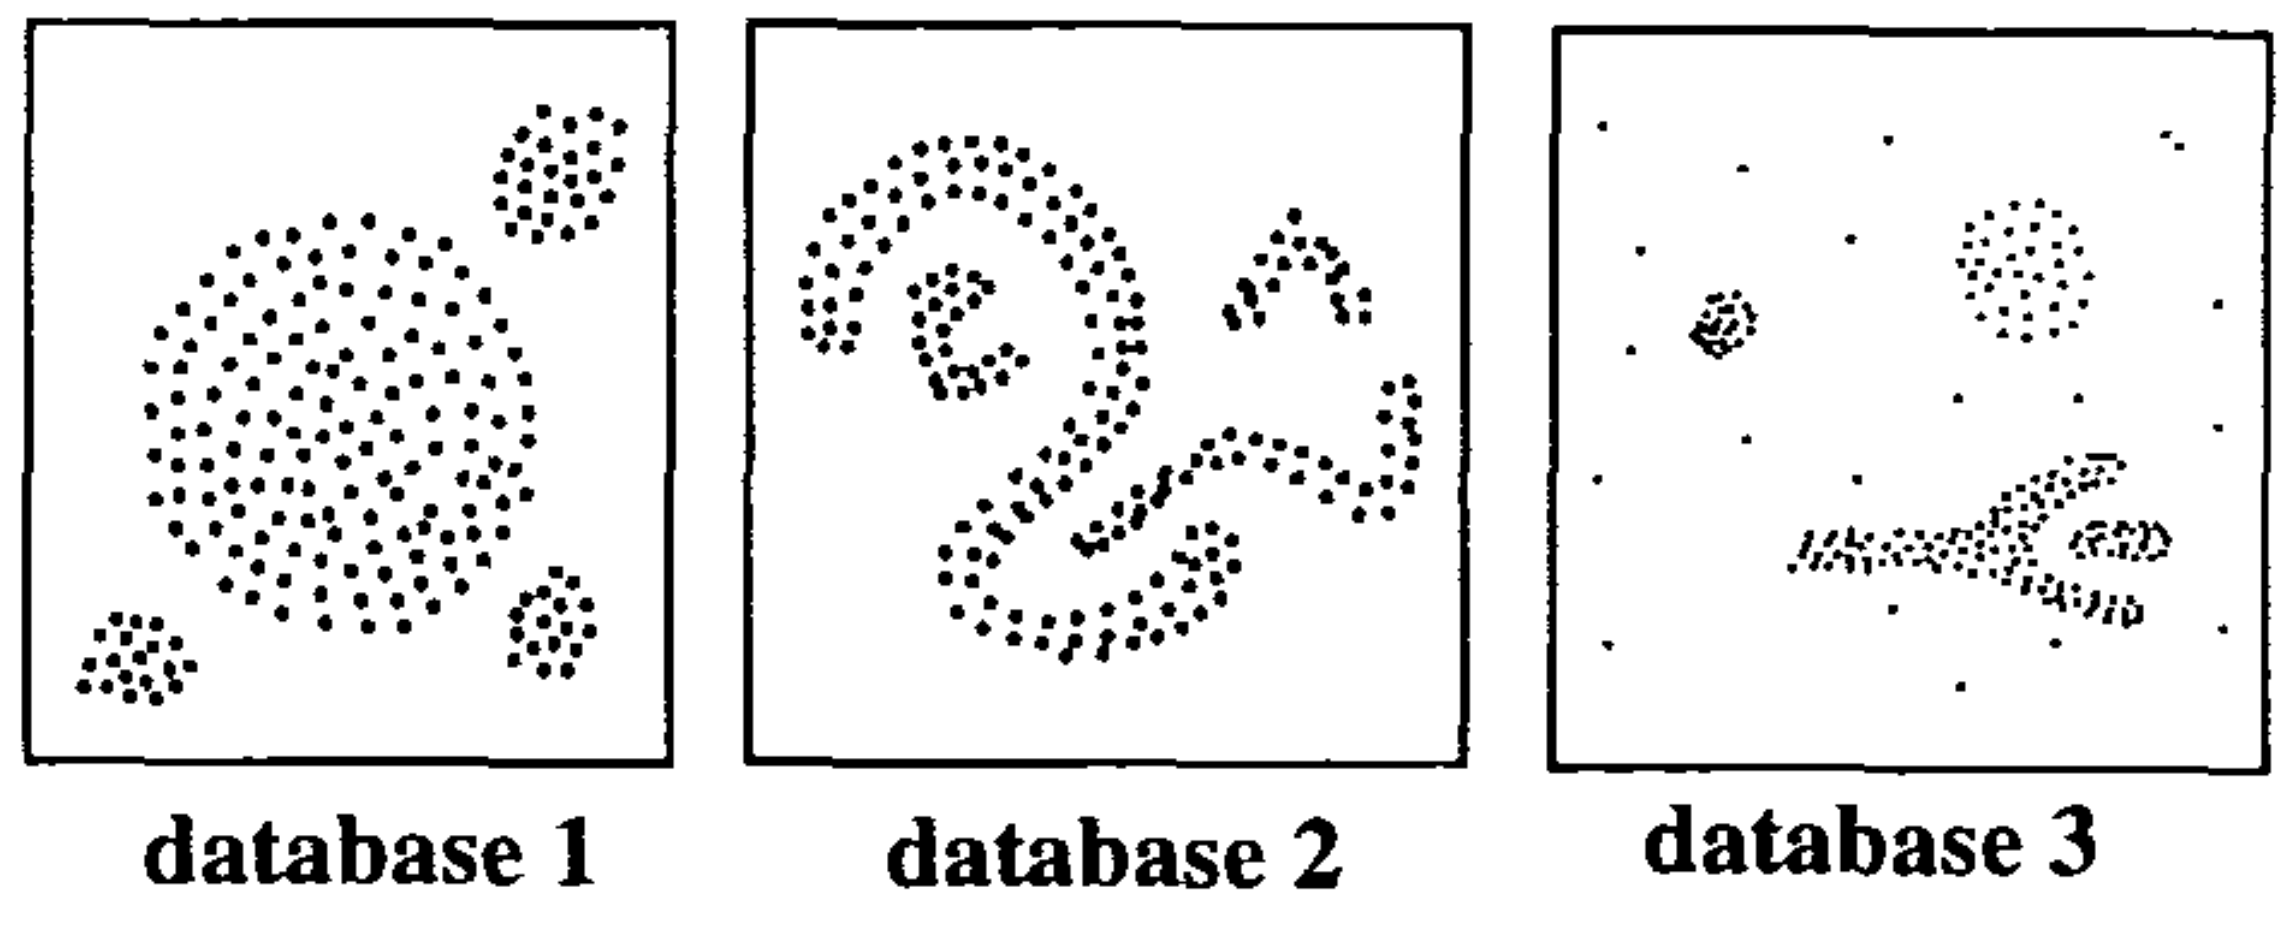
\includegraphics[width=\textwidth]{images/dbscan-clusters.png}
    \caption{Data from three different databases with very distinct cluster shapes. Database \#1 has very round clusters which would identified correctly with K-means whereas database \#2 and \#3 have clusters which would require a different clustering approach.}
    \label{fig:my_label}
\end{figure}

GPS data has a higher density inside clusters than outside the clusters and the density in noisy areas is lower than density in clusters. Here, \textit{noisy} refers to points that are spread randomly within some area and do not cluster around a centroid.

The DBSCAN algorithm will, given a set of geo-spatial data points and a small set of parameters, find these dense clusters as well as noisy data points, where the clusters correspond to places and the noisy data points are outliers which do not belong to a place. The output of the algorithm is a labelling of each point in the input dataset as either belonging to a cluster or being a noisy data point.

\section{Mathematical Definitions}

The DBSCAN paper defines a \textit{Neighbourhood} as a collection of data points within some radius, i.e. an area defined by a distance function. Within a Neighbourhood, two types of points can reside: \textit{Core points}, that is, points which are inside in the neighbourhood, and \textit{Border points } which lie on the edge of the neighbourhood and delimit it. 

\subsubsection*{Definition 1: Epsilon Neighbourhood}
An Epsilon Neighbourhood is a Neighborhood defined on a point $p$ which includes all the points $q$ which are inside a radius of $\epsilon$ of $p$, formally this is defined as $N_{\epsilon} (p) = q \in D \quad|\quad dist(p,q) \leq \epsilon$

\textit{Note: The $N_{\epsilon}$ of a border point contains much fewer points than that of a core point. }

We Require for all points $p$ and a given cluster $C$: There must be a a point $q \in C$ st. $p \in N_{\epsilon}(q)$ of and $N_{\epsilon}(q)$ contains at least $T_{min}$ points where $T_{min}$ is a parameter which defines the minimum number of points required.

\subsubsection*{Definition 2: Directly Density-Reachable (DDR)}
A point $p$ is DDR from point $q$ wrt. the parameters $\epsilon$ and $T_{min}$ if
1. $p \in N_{\epsilon}(q)$
2. $|N_{\epsilon}(q)| \geq T_{min}$ (\textit{Core Point Condition})

This implies a border point $p$ may be DDR from a core point $q$, but it is likely not true the other way around, since $N_{\epsilon}(p)$ is probably smaller than the minimum amount of points needed to satisfy the \textit{Core Point Condition}.

\subsubsection*{Definition 3: Density-Reachable (DR)}
A point $p$ is DR from a point $q$ if:
There is a chain of points $p_1, ..., p_n$ , where $p_1 = q$ and $p_n = p$, such that $p_{i+1}$ is DDR from $p_i$.
This is denoted $DR(p,q)$

\textit{Note that, only symmetric for core points, but not symmetric in general and that two border points from the same cluster may not be DR due to them not satisfying the Core Point Condition.}

\subsubsection*{Definition 4: Density-Connected (DC)}
A point $p$ is DC to $q$ if there exists a point $o$ st. both $p$ and $q$ are DR from $o$, this is denoted $DC(p,q)$. DC is a symmetric relation meaning that $DC(p,q) \iff DC(q,p)$.

\subsubsection*{Definition 5: Cluster}
A cluster is a set of DC points which is have maximal Density-Reachability. 

That is, for all points $p,q$, if $p \in C$ and $DR(p,q)$ then $q \in C$
For all points $p,q \in C$: $p$ is Density-Connected to $q$, i.e. $DC(p,q) $.

The parameters $\epsilon$ and $T_{min}$ are global, i.e. the same for all clusters.

\subsubsection*{Definition 6: Noise}
Noisy points are defined as all the points $p$ for which $p \in D \wedge p \notin C_i$ for all clusters $i = 1,...,N$, that is, all the points not belonging to any cluster.

\subsubsection*{Lemma 1}
Let $p$ be a point in $D$ for which the core point condition holds. Then, the set $O$ which is the set of DR points from $p$ (wrt. the parameters) is a cluster wrt. to the parameters. This means, a cluster $C$ contains exactly the points which are DR from an arbitrary core point of $C$.

\subsubsection*{Lemma 2}
Let $C$ be a cluster wrt. to the chosen parameters and let $p$ be a core point in $C$, then it holds that $C = O$.

\subsection{Choice of Parameters}
There is no reliable way of knowing the parameters $\epsilon$ and $T_{min}$ for each cluster in advance. Instead, the parameters are determined based on the least dense cluster, and used globally for all clusters.

\section{The DBSCAN Algorithm}
Start with a random point $p$ and get all DR points from $p$ wrt. the parameters.
Given $p \in D$: 
\begin{itemize}
\item If $p$ is a core point, then $O = DR(p)$ is a cluster (\textit{Lemma 2}).
\item Otherwise, if $p$ is a border point, then $DR(p) = \{\}$ and the algorithm proceeds to the next point $q$
\end{itemize}
Once all points have been considered, the algorithm terminates. 

Note: Since the parameters are global, the algorithm may merge two clusters according to \textit{Definition 5} if two clusters are close to each other (even if the two densities are different).
